\chapter{Introduzione}
\label{cap:introduzione}

Le linee guida della World Health Organization (WHO) indicano che la malattia SARS-CoV-2 coronavirus ed in particolare la sua recente forma COVID-19 si trasmettono principalmente attraverso il contatto corporeo e tramite le goccioline respiratorie (droplets). La trasmissione per contatto avviene quando le mani contaminate toccano le membrane mucose della bocca, del naso o gli occhi. In particolare, per quanto riguarda il COVID-19 è stimato che la maggior parte dell'infezione avviene proprio attraverso il contatto delle mani con le superfici contaminate \cite{santarpia2020aerosol}. Per questo motivo una delle misure più importanti che una persona può mettere in pratica per prevenire la trasmissione di germi è prendersi cura dell'igiene delle proprie mani.

Per garantire un'igiene delle mani sufficiente la WHO suggerisce di lavarle accuratamente con acqua e sapone oppure sanificarle utilizzando una sostanza a base di alcool.
Le procedure suggerite in Figura \ref{fig:who-steps} sono composte da molteplici passaggi ciascuno di diversa durata; lavare le mani con acqua e sapone prevede undici step per una durata complessiva fra 
i 40 secondi e i 60 secondi mentre la sanificazione è formata solo da 8 passaggi di durata fra i 20 secondi e i 30 secondi. 
La WHO inoltre indica la sanificazione delle mani con l'alcool come decontaminazione di routine, mentre raccomanda il lavaggio con acqua e sapone nei casi in cui le mani sono visibilmente sporche.
Nonostante la provata efficienza di questi due metodi un numero significativo di persone non li mette in pratica a causa della loro difficoltà d'implementazione e si limitano a lavare le loro mani come hanno sempre fatto.

\begin{figure}[!htb]
    \centering
    \begin{subfigure}{.45\textwidth}
        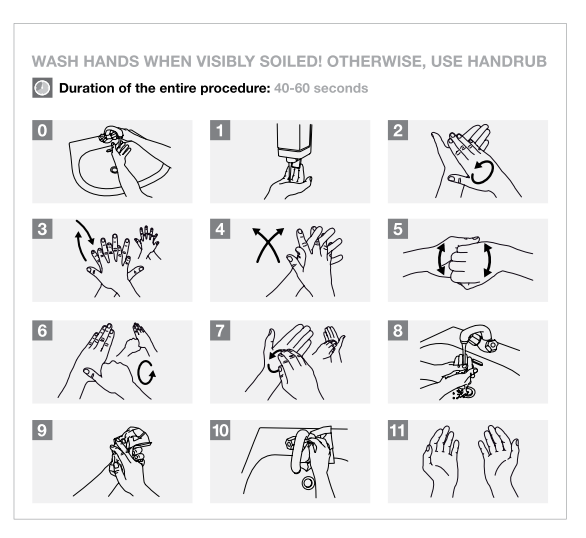
\includegraphics[width=\textwidth]{figure/handwash.png}
        \caption{lavaggio delle mani}
        \label{fig:handwash}
    \end{subfigure}
    \begin{subfigure}{.45\textwidth}
        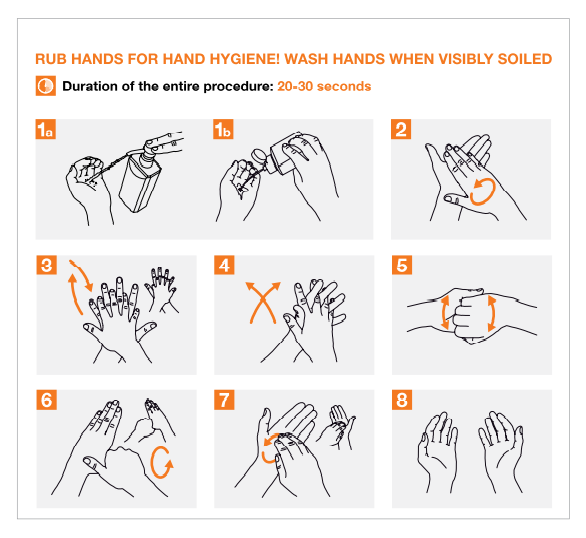
\includegraphics[width=\textwidth]{figure/handsan.png}
        \caption{sanificazione delle mani}
        \label{fig:handsan}
    \end{subfigure}
    \caption{Procedure suggerite dalla WHO per il corretto lavaggio (\subref{fig:handwash}) e sanificazione (\subref{fig:handsan}) delle mani.}
    \label{fig:who-steps}
\end{figure}

I dispositivi indossabili, come i moderni smartwatch, sono equipaggiati con diversi sensori in grado di misurare continuamente i parametri caratteristici del movimento dei nostri corpi; un esempio è quello di Wang et al.\cite{wang2020accurate} che nel 2020 hanno misurato l'accuratezza di braccialetti indossabili con all'interno accelerometri, giroscopi ed elettrodi per elettromiografia (sEMG) nell'identificare e monitorare le procedure di lavaggio e sanificazione delle mani suggerite dalla WHO raggiungendo un'accuratezza superiore al 96\%.
Prima di loro, molti altri autori hanno dimostrato l'efficacia dei dispositivi indossabili nel classificare attività umane generali come ad esempio la corsa, la camminata, salire o scendere le scale, saltare e sedersi\cite{zhang2013human}\cite{sztyler2016body}\cite{sztyler2017position}\cite{bhat2018online}\cite{koping2018general}\cite{lattanzi2022exploring}.

La facile reperibilità di data-set di grandi dimensioni per il riconoscimento di attività umane, assieme ai recenti sviluppi nel deep learning, hanno portato ad incredibili risultati aumentando significativamente l'accuratezza nella classificazione delle attività generali che ora raggiunge valori anche del 99\%\cite{cheng2010active}\cite{singh2017convolutional}\cite{hassan2018robust}\cite{hou2020study}.

Quando non si seguono le procedure raccomandate dalla WHO l'attività di lavare le mani è eseguita in maniera molto personale il che ci porta ad ottenere dei dati che definiamo completamente non strutturati.
La presenza di dati non strutturati, assieme alle performance dei sistemi di machine learning porta alla nascita di nuovi problemi etici che non possono essere trascurati \cite{muller2021ten}. Inoltre, a differenza delle attività che coinvolgono l'intero corpo, come la camminata o la corsa, lavare le mani richiede movimenti molto precisi di muscoli, tendini e ossa delle dita che non è scontato siano facilmente riconoscibili partendo dai dati raccolti, dal polso del soggetto tramite un comune smartwatch. 

Per i motivi sopra citati in questa tesi ci concentreremo sul riconoscimento dei lavaggi e delle sanificazioni delle mani partendo da dati non strutturati con lo scopo di investigare l'accuratezza nella 
classificazione di un sistema basato su smartwatch capace di monitorare l'igiene delle mani della gran parte della popolazione. In particolare, introduciamo uno studio sperimentale estensivo volto a valutare l'abilità dei sistemi di machine learning di distinguere i gesti di lavaggio e sanificazione dal resto delle attività che ogni persona compie giornalmente senza l'utilizzo di strumenti invasivi, ma facendo unicamente affidamento su dispositivi indossabili comuni come smartwatch disponibili commercialmente.

Nei capitoli seguenti si parlerà in maniera più approfondita dei sistemi di machine learning presi in esame descrivendo lo stato dell'arte in questo ambito, illustrando i metodi e le relative scelte fatte durante lo svolgimento della ricerca e presentando i risultati delle valutazioni sperimentali dei diversi modelli sia su PC che sul dispositivo embedded utilizzato come benchmark: l'HEXIWEAR. Infine si presenterà lo sviluppo di un'applicazione per il monitoraggio dell'igiene delle mani creata per lo smartwatch HEXIWEAR e che fa largo utilizzo dei modelli di machine learning per il riconoscimento degli eventi.

Da parte di questo lavoro di tesi è stato prodotto un articolo scientifico pubblicato nel 2022 su un'importante rivista specializzata\cite{lattanzi2022unstructured}.
